%versi 2 (8-10-2016)
\chapter{Implementasi dan Pengujian}
\label{chap:implementasi dan pengujian}

\def\scl{1}
% \def\leg{\legend{Switching,Homotopic,Buffer*Length,Length}}
\def\leg{} 
\def\std{none}
\def\ymin{}
\def\ymax{}

Bab ini terdiri dari implentasi perangkat keras maupun lunak yang telah dibahas pada bab \ref{chap:perancangan}. Pada bab ini juga akan dibahas pengujian yang dilakukan atas aplikasi yang dibangun, dipandang dari hasil pengujian perangkat keras maupun pengujian perangkat lunak yang digunakan. Selain hal yang telah disebutkan diatas, bab ini juga akan membahas kendala dan kesulitan yang dialami selama perancangan sampai pengujian aplikasi dilakukan. 

\section{Implementasi}
\label{sec:skripsi} 
    Implementasi merupakan kegiatan atau tindakan yang dilakukan berdasarkan hasil perancangan tertentu, yang bertujuan untuk mencapai tujuan tertentu. Pada aplikasi yang dibangun, implementasi dilakukan di tanah persawahan dengan tujuan untuk menguji aplikasi yang dibangun serta mendapatkan data unsur-hara tanah dari hasil \textit{sensing} yang dilakukan selama implementasi.

   \subsection{Lingkungan Implementasi}
   Berikut adalah perangkat keras yang digunakan untuk melakukan implementasi, juga perangkat lunak yang dioperasikan pada perangkat keras tersebut.
   
   \begin{itemize}
       \item Laptop
       
       Spesifikasi laptop yang digunakan dalam implementasi aplikasi adalah sebagai berikut.
       
       \begin{itemize}
           \item Perangkat Keras
                \begin{itemize}
                    \item \textit{Processor} : Intel(R) Core(TM) i5-7200 
                    \item \textit{Memory} : 12288MB
                \end{itemize}
           
           \item Perangkat Lunak
                \begin{itemize}
                    \item \textit{Operation System} : Windows 10 Home 64-bit
                    \item \textit{Remote access (CLI)} : PuTTy
                    \item \textit{Remote access (GUI)} : VNC
                    \item  IDE : Arduino IDE 
                \end{itemize}
       \end{itemize}
       
        
       
       \item Raspberry Pi 3 B+
       
       Spesifikasi Raspberry Pi yang berperan sebagai \textit{base station} dalam implementasi aplikasi adalah sebagai berikut.
       
       \begin{itemize}
           \item Perangkat Keras
                \begin{itemize}
                    \item \textit{Processor} : 1.4GHz 64-bit quad-core 
                    \item \textit{Memory} : 1000MB
                    \item \textit{Power} : 2.5A
                \end{itemize}
           
           \item Perangkat Lunak
                \begin{itemize}
                    \item \textit{Operation System} : Raspbian Pi
                    \item \textit{Remote access (GUI)} : VNC
                    \item \textit{Browser} : Chromium
                    \item \textit{PHP Version} : 7.0.1
                    \item \textit{Framework} : Laravel 8.x
                \end{itemize}
       \end{itemize}
       
       \item \textit{Powerbank}
       
       \textit{Powerbank} yang berperan sebagai pemberi daya \textit{base station} untuk kebutuhan implementasi atau pengujian diluar ruangan. Spesifikasi \textit{powerbank} yang digunakan adalah sebagai berikut.
       
            \begin{itemize}
                \item Model : Anker Astro E1
                \item Capacity : 6700mAh
                \item Input/Output : 5V=1A / 5V=2A
            \end{itemize}
       
      
       \item Arduino Mega 2560
       
            \begin{itemize}
                \item \textit{Chip} : ATMEGA2560
                \item \textit{Memory} : 256KB
                \item Jumlah I/O : 54
            \end{itemize}
        
       
       \item Sensor \textit{sensing}
       
       Sensor \textit{sensing} yang terhubung dengan perangkat Arduino terdiri dari sensor kelembaban tanah, sensor keasaman tanah (pH tanah), sensor suhu dan kelembaban udara, sensor suhu tanah, dan perangkat X-Bee untuk komunikasi. 
       
   \end{itemize}
   
   \subsection{Hasil Implementasi}
  
   Berdasarkan pembahasan pada bab \ref{chap:perancangan}, terdapat dua buah kelas yang dilakukan secara terpisah, yaitu pemograman pada node sensor (Kelas Node Sensor) yang dilakukan menggunakan bahasa Arduino dan pemrograman pada \textit{base station} (Kelas \textit{Base-Station}) yang dilakukan menggunakan bahasa Python.
   
   \subsubsection{Kelas Node Sensor}
   
   Pada kelas Node sensor terdapat barisan code program '\#include' yang berfungsi untuk mengimport library-library. Barisan kode tersebut diperlukan agar sensor \textit{sensing} dapat melakukan pengambilan data. Setelah kode program untuk mengimport library, maka terdapat banyak inialisasi untuk setiap sensor \textit{sensing} yang terhubung dengan perangkat Arduino.
   
   Pada kelas ini terdapat dua buah methods default Arduino yaitu setup dan loop. Method setup merupakan method yang pertama kali dieksekusi oleh program ketika mendapat power up. Method setup akan menginformasikan serial komunikasi (dalam aplikasi ini baut 9600) juga menginialisasi pin-pin yang akan digunakan untuk melakukan transfer data hasil \textit{sensing} maupun pengiriman pesan. 
   
   
   \begin{lstlisting}[label=setup, language=C, caption=Metode setup(), numbers=none]
        void setup(){
             Serial.begin(9600);
             dht.begin();
            
             // jadikan pin power sebagai output
              pinMode(powerPin, OUTPUT);
            
              // initialize digital pin LED_BUILTIN as an output.
              pinMode(LED_BUILTIN, OUTPUT);
               
              // default bernilai LOW
              digitalWrite(powerPin, LOW);
            
              // mulai komunikasi serial
              xbee.begin(9600);
        }
    \end{lstlisting}

    
    \begin{itemize}
        \item Melakukan \textit{sensing}
        
        Perangkat Arduino yang berperan sebagai node sensor akan mengambil data yang dilakukan oleh sensor \textit{sensing} dan disimpan sementara sebelum dikirimkan ke \textit{base station}.
        
        Pada perangkat ini terdapat beberapa pemrograman method untuk mengambil hasil \textit{sensing} dari setiap sensor \textit{sensing} yang terhubung dengan perangkat Arduino.
        
         
        
        \begin{itemize}
            \item Method loop
            
             Method loop yang akan terus dieksekusi selama Arduino memiliki daya untuk tetap menyala. Method loop pada kelas ini dijadikan sebagai wrapper, yang merupakan method penampung hasil method-method lainnya. Method loop juga berperan untuk menampilkan data hasil \textit{sensing} ke aplikasi sebelum paket dikirimkan ke \textit{base station}.
             
             \begin{lstlisting}[label=loop, language=C, caption=Metode loop(), numbers=none]
   
            void loop(){
               Serial.println("");
               Serial.print("Node pengiriman: ");
               Serial.println(node1);
               Serial.print("Kelembaban Tanah: "); 
               Serial.print(bacaSensorKelembabanTanah());
               Serial.println("^-10 %");
               Serial.print("Kelembaban Udara: ");
               Serial.print(bacaSensorKelembabanUdara());
               Serial.println(" %");
               Serial.print("Suhu Tanah: ");
               Serial.print(bacaSensorSuhuTanah());
               Serial.println(" C");
               Serial.print("Suhu Udara: ");
               Serial.print(bacaSensorSuhuUdara() );
               Serial.println(" C");
               Serial.print("Kadar Keasaman Tanah (pH): ");
               Serial.println(bacaSensorPhTanah());
               Serial.println("");
               Serial.println(WrapperStatusNodeDanSensing());
               
        \end{lstlisting}
        
        
            \item Method bacaSensorKelembabanTanah
            
            Method ini berfungsi untuk mendapatkan data hasil \textit{sensing} kelembaban tanah, dari sensor \textit{sensing} yang tertancap di tanah yang diuji.
            
            \begin{lstlisting}[label=bacaSensorKelembabanTanah, language=C, caption=Metode bacaSensorKelembabanTanah(), numbers=none]
            
            float bacaSensorKelembabanTanah() {
              // hidupkan power
              digitalWrite(powerPin, HIGH);
              delay(2000);
              
              // baca nilai analog dari sensor
              int nilaiSensor = analogRead(sensorPin);
              digitalWrite(powerPin, LOW);
              
              // makin lembab maka makin tinggi nilai outputnya
              // konversi sensor kelembaban tanah (analog ke digital)
              return (1023 - nilaiSensor)/10;
            }
            
            
            \end{lstlisting}
            
            \item Method bacaSensorKelembabanUdara
            
            Method bacaSensorKelembabanUdara memiliki peran untuk mengambil data kelembaban udara dari area persawahan yang diuji.
            
            \begin{lstlisting}[label=bacaSensorKelembabanUdara, language=C, caption=Metode bacaSensorKelembabanUdara(), numbers=none]
            
            float bacaSensorKelembabanUdara(){
              float kelembaban = dht.readHumidity();
              return kelembaban;
            }
            
            \end{lstlisting}
            
            \item Method bacaSensorSuhuTanah
            
            Method ini berfungsi untuk mengetahui suhu tanah yang diuji, dengan cara mengambil data dari hasil \textit{sensing} yang dilakukan sensor \textit{sensing}, yang ditancapkan ke tanah yang dilakukan pengamatan.
            
            \begin{lstlisting}[label=bacaSensorSuhuTanah, language=C, caption=Metode bacaSensorSuhuTanah(), numbers=none]
            
            float bacaSensorSuhuTanah(){
               sensorSuhuTanah.requestTemperatures();
               float suhuTanah = sensorSuhuTanah.getTempCByIndex(0);
               return suhuTanah;   
            }
            
            \end{lstlisting}
            
            \item Method bacaSensorSuhuUdara
            
            Seperti method bacaSensorSuhuTanah, method bacaSensorSuhuUdara juga mengambil data suhu. Namun data suhu yang diambil adalah suhu udara dari area yang dilakukan pengamatan.
            
            \begin{lstlisting}[label=bacaSensorSuhuUdara, language=C, caption=Metode bacaSensorSuhuUdara(), numbers=none]
            
            float bacaSensorSuhuUdara(){
              float suhu = dht.readTemperature();
              return suhu;
            }
            
            \end{lstlisting}
            
            \item Method bacaSensorPhTanah
            
            Method bacaSensorPhTanah berfungsi untuk mendapatkan data tingkat keasaman tanah yang diuji. Method ini akan menerima data dari sensor \textit{sensing} yang ditancapkan ditanah dan melakukan konversi sinyal sebelum dikirimkan ke \textit{base station}.
            
            \begin{lstlisting}[label=bacaSensorPhTanah, language=C, caption=Metode bacaSensorPhTanah(), numbers=none]
            
            float bacaSensorPhTanah(){
              //mengambil data \textit{sensing} sensor
              sensorValue = analogRead(analogInPin);
            
              //Mathematical conversion from ADC to pH
              //Konversi analog menjadi digital
              //rumus didapat berdasarkan datasheet 
              phValue = (-0.0693*sensorValue)+7.3855;
            
              return phValue*-1;
            }
            
            \end{lstlisting}
            
            \item Method conversiDataFloatToString
            
            Method conversiDataFloatToString berfungsi untuk mengubah seluruh hasil data \textit{sensing} yang umumnya berjenis data float menjadi string agar dapat dikirimkan ke baseStation melalui method transmisiPengiriman.
            
            \begin{lstlisting}[label=conversiDataFloatToString, language=C, caption=Metode conversiDataFloatToString(), numbers=none]
            
            String conversiDataFloatToString(){
              String kelembabanTanah =
                String(bacaSensorKelembabanTanah());
              String kelembabanUdara =
                String(bacaSensorKelembabanUdara());
              String suhuTanah = String(bacaSensorSuhuTanah());
              String suhuUdara = String(bacaSensorSuhuUdara());
              String phTanah = String(bacaSensorPhTanah());
              String res = node2+"|"+kelembabanTanah+"|"+
              kelembabanUdara+"|"+suhuTanah+"|"+
              suhuUdara+"|"+phTanah+"|"+
              WrapperStatusNodeDanSensing();
              return res;
            }
            
            \end{lstlisting}
            
            % \item Method displayInfoGIS
            
            % Method displayInfoGIS berfungsi untuk mengambil data lokasi node sensor dan mengembalikannya dalam bentuk nilai lintang dan bujur.
            
            % \begin{lstlisting}[label=displayInfoGIS, language=C, caption=Metode displayInfoGIS(), numbers=none]
            
            % void displayInfoGIS(){
            %   Serial.print(F("Location: ")); 
            %   if (gps.location.isValid())
            %   {
            %     Serial.print(gps.location.lat(), 6);
            %     Serial.print(F(","));
            %     Serial.print(gps.location.lng(), 6);
            %   }
            %   else
            %   {
            %     Serial.print(F("INVALID"));
            %   }
              
            %   Serial.println();
            % }
            
            % \end{lstlisting}
            
            
        \end{itemize}
        
        \item Melakukan Respon terhadap perintah \textit{Base Station}
        
        Node dapat melakukan instruksi yang dikirim oleh \textit{base station}, dan dapat mengirim respon untuk membalas perintah tertentu yang dikirimkan. Barisan kode dibawah ini terdapat didalam void loop, sehingga aplikasi akan menunggu input instruksi secara berkala.
        
        \begin{lstlisting}[label=transmisiPengiriman, language=C, caption=Respon Perintah Base Station, numbers=none]
        
        /* ========= Perintah dari Base Station=========== */
         //terdapat input perintah dari base station
          if (xbee.available()) { 
            boolean adaPerintah = true;
            char temp= xbee.read();
            if(temp=='a'){ //mulai sensing
              String pesan = conversiDataFloatToString();
              transmisiPengiriman(pesan);
            }
            else if(temp == 'b'){ //check status
              String pesan = WrapperStatusNodeDanSensing();
              transmisiPengiriman(pesan);
             }
             else if(temp == 'c'){ //stop sensing
                adaPerintah = false;
                while(xbee.available()){ //cek perintah base station
                    if(adaPerintah == false){ 
                    //selama ga ada perintah >> kunci loop
                       delay(5000);
                      }
                    else{
                      //keluar kunci loop dan kembali ke void loop
                      break; 
                    }
                 } 
                
              }
          }
        
        \end{lstlisting}
        
        
        \item Konversi data Analog menjadi Digital
        
        Beberapa perangkat sensor \textit{sensing} memiliki spesifikasi pengambilan data secara analog. Perangkat sensor \textit{sensing} dengan pengambilan data analog adalah sensor keasaman tanah (pH Tanah) dan kelembaban tanah. Oleh karena itu, diperlukan konversi tipe data dari analog menjadi digital sebelum dikirimkan ke \textit{base station}.
        
        \begin{lstlisting}[label= bacaSensorPhTanah, language=C, caption=Metode  bacaSensorPhTanah(), numbers=none]
   
        float bacaSensorPhTanah(){
          //mengambil data sensing sensor
          sensorValue = analogRead(analogInPin);
        
          //Mathematical conversion from ADC to pH
          //Konversi analog menjadi digital
          //rumus didapat berdasarkan datasheet 
          phValue = (-0.0693*sensorValue)+7.3855;
        
          return phValue*-1;
        }
        
        \end{lstlisting}
        
        \begin{lstlisting}[label= bacaSensorKelembabanTanah, language=C, caption=Metode  bacaSensorKelembabanTanah(), numbers=none]
   
        float bacaSensorKelembabanTanah() {
          // hidupkan power
          digitalWrite(powerPin, HIGH);
          delay(2000);
          
          // baca nilai analog dari sensor
          int nilaiSensor = analogRead(sensorPin);
          digitalWrite(powerPin, LOW);
          
          // makin lembab maka makin tinggi nilai outputnya
          // konversi sensor kelembaban tanah (analog ke digital)
          return (1023 - nilaiSensor)/10;
        }
        
        \end{lstlisting}
        
        
        \item Mengirim status node dan status \textit{sensing}
        
        Selain mengirimkan data hasil \textit{sensing}, node sensor juga mengirim status aktif dari node dan status \textit{sensing}. Untuk mengetahui nilai status sensor node, method checkstatusnode akan mengembalikan nilai \textit{true} jika \textit{online}, dan \textit{false} jika \textit{offline}.
        
        \begin{lstlisting}[label=checkStatusNode, language=C, caption=Metode checkStatusNode(), numbers=none]
        
        boolean checkStatusNode(){
           if(checkStatusSensing()==true){
              return true;
            }
            else{ //check lampu indikator 'on' Arduino
              if(digitalRead(LED_BUILTIN == HIGH)){
                return true;  
              }
              else{
                return false;  
              }
            }
          }
        
        \end{lstlisting}
        
        Untuk mengetahui nilai status \textit{sensing}, method checkStatusSensing akan dieksekusi. Seperti method checkStatusNode, checkStatusSensing akan mengembalikan nilai \textit{true} apabila node sendang melakukan pengamatan atau \textit{sensing}, dan mengembalikan nilai \textit{false} apabila tidak melakukan pengamatan atau \textit{sensing}.
        
        \begin{lstlisting}[label=checkStatusSensing, language=C, caption=Metode checkStatusSensing(), numbers=none]
        
      boolean checkStatusSensing(){
          boolean kelembabanTanah = false;
          boolean kelembabanUdara = false;
          boolean suhuTanah = false;
          boolean suhuUdara = false;
          
          // ph Tanah tidak memiliki value pasti- 
          //ketika sensor bermasalah
          boolean phTanah = true; 
          
          boolean isSensing = false;
          
            if(bacaSensorKelembabanTanah()!=1023.0){ 
            //1023.00 adalah value yang didapatkan-
            //jika sensor suhu tanah bermasalah
                kelembabanTanah = true;
            }
            if(isnan(bacaSensorKelembabanUdara())==false){ 
            //bukan nan (mengembalikan value), 
            //jika bermasalah value = nan
                kelembabanUdara = true;
            }
            if(bacaSensorSuhuTanah()!=-127.00){ 
            //-127.00 adalah value yang didapatkan- 
            //jika sensor suhu tanah bermasalah
                suhuTanah = true;
            }
            if(isnan(bacaSensorSuhuUdara())==false){ 
            //bukan nan (mengembalikan value), 
            //jika bermasalah value = nan
                suhuUdara = true;
            }
        
            if((kelembabanTanah&&kelembabanUdara&&
            suhuTanah&&suhuUdara&&phTanah)==true){
              isSensing = true;
            }
            return isSensing;
        }
        
        \end{lstlisting}
        
        
        \item Mengirim data hasil \textit{sensing}
        
        Setelah data hasil \textit{sensing} didapatkan dan di konversi dengan baik, maka node sensor harus mengirimkan data hasil \textit{sensing} tersebut sebelum melakukan pengambilan data \textit{sensing} berikutnya.
        
        \begin{lstlisting}[label=transmisiPengiriman, language=C, caption=Metode transmisiPengiriman(), numbers=none]
        
        String transmisiPengiriman(String pesan){
          xbee.print(pesan);
        }
        \end{lstlisting}
        
        
        
    \end{itemize}
   
   Kode program kelas ini secara lengkap dapat dilihat pada lampiran \ref{lamp:A}.
   
   \subsubsection{Kelas Base Station}
   
   Pada kelas \textit{base station} terdapat dua buah method utama yang akan selalu dieksekusi yaitu getDataSensing dan sentDataSensing. 
   
   
   \begin{itemize}
       \item Menerima data hasil \textit{sensing}
       
       Method getDataSensing berperan untuk mengambil data yang dikirimkan oleh node sensor yang berkomunikasi menggunakan perangkat X-bee dari recevier (node sensor) ke coordinator (\textit{base station}). Method getDataSensing juga berfungsi untuk menampilkan hasil data \textit{sensing} yang dikirimkan oleh node untuk menunjukan bahwa paket telah diterima dan siap untuk dikirimkan dan disimpan di internet (localhost).
   
   \begin{lstlisting}[label=getDataSensing, language=Python, caption=Metode getDataSensing(), numbers=none]
    
    def getDataSensing(dataSensing):
    # Data yang dikirim Arduino (String)
    # "Node 1"+"|"+kelembabanTanah+"|"+kelembabanUdara+"|"+suhuTanah+"|"
    #+suhuUdara+"|"+phTanah+"|"+statusNode+"|"+"statusSensing";
    
    potongData = dataSensing.split("|")
    
    if len(potongData) > 1:
        nodeSensing = potongData[0]
        kelembabanTanah = potongData[1]
        kelembabanUdara = potongData[2]
        suhuTanah = potongData[3]
        suhuUdara = potongData[4]
        phTanah = potongData[5]
        statusNode = potongData[6]
        statusSensing = potongData[7]

        waktuSensing = datetime.datetime.now()
        waktuSensing = waktuSensing.strftime('%Y-%m-%d %H:%M:%S')
        
        return nodeSensing,kelembabanTanah,kelembabanUdara,
        suhuTanah,suhuUdara,phTanah,statusNode,statusSensing,
        waktuSensing
    \end{lstlisting}
    
        \item Menyamakan waktu node
        
        Setiap node akan mengirimkan hasil \textit{sensing} beserta waktu data hasil \textit{sensing} diterima oleh \textit{base station}.
        
        \begin{lstlisting}[label=getDataSensing, language=Python, caption=Metode getDataSensing(), numbers=none]
        
        waktuSensing = datetime.datetime.now()
        waktuSensing = waktuSensing.strftime('%Y-%m-%d %H:%M:%S')
            
        \end{lstlisting}
       
       \item Menyimpan data hasil \textit{sensing}
       
        Setelah data diterima dengan baik oleh \textit{base station}, maka \textit{base station} akan meneruskan data hasil \textit{sensing} tersebut ke basisdata (internet) yang dalam pembangunan aplikasi ini tersimpan di localhost.
    
    \begin{lstlisting}[label=sentDataSensing, language=Python, caption=Metode sentDataSensing(), numbers=none]
    
    def sentDataSensing(dataSensing):
    db = mysql.connector.connect(
        host = 'localhost',
        database = 'Skripsi II',
        user = 'admin',
        password = 'root',
        pool_name = 'mypool',
        pool_size = POOL_SIZE+1
    )

    nodeSensing = dataSensing[0]
    kelembabanTanah = dataSensing[1]
    kelembabanUdara = dataSensing[2]
    suhuTanah = dataSensing[3]
    suhuUdara = dataSensing[4]
    phTanah = dataSensing[5]
    statusNode = dataSensing[6]
    statusSensing = dataSensing[7]
    

    kelembabanTanahFlt = float(kelembabanTanah)
    kelembabanUdaraFlt = float(kelembabanUdara)/10.0
    suhuTanahFlt = float(suhuTanah)
    suhuUdaraFlt = float(suhuUdara)
    phTanahFlt = float(phTanah)

    getNodeNumber = nodeSensing[len(nodeSensing)-1]
    getNodeNumberInt = int(getNodeNumber)

    waktuSensing = datetime.datetime.now()
    waktuSensing = waktuSensing.strftime('%Y-%m-%d %H:%M:%S')

    jenisTanah = "irigasi"

    #cursor digunakan untuk memasukan data ke mysql, dan eksekusi query
    cursor = db.cursor(buffered=True)

    queryTanah = ("INSERT INTO sensing(waktu_sensing,ph_tanah,
    suhu_tanah,kelembaban_tanah,suhu_udara,
    kelembaban_udara,kode_petak,jenis_tanah) 
    VALUES (%s,%s,%s,%s,%s,%s,%s,%s)")
    
    queryInputTanah = (waktuSensing,phTanahFlt,suhuTanahFlt,
    kelembabanTanahFlt,suhuUdaraFlt,
    kelembabanUdaraFlt,getNodeNumberInt,
    jenisTanah)

    cursor.execute(queryTanah,queryInputTanah)

    queryNode2 = ("UPDATE nodesensor SET status_node = %s ,
    status_sensing = %s, waktu_node = %s 
    WHERE kode_node = %s")
    queryInputNode2 = (statusNode,statusSensing,waktuSensing,
    getNodeNumber)

    
    cursor.execute(queryNode2,queryInputNode2)
    
    db.commit()
    cursor.close()
    db.close()
   
    \end{lstlisting}
       
   \item Menampilkan opsi fitur aplikasi (main menu)
   
   Ketika aplikasi admin pertama kali buka, aplikasi akan menampilkan opsi fitur aplikasi yang dapat dipilih oleh Admin. Opsi fitur yang dapat dipilih admin antara lain, check status node, mulai \textit{sensing}, stop \textit{sensing}, dan matikan aplikasi \textit{base station}. Untuk mengeksekusi opsi yang diberikan admin dapat menginput nomor opsi yang ingin dieksekusi pada aplikasi 
   
   \begin{lstlisting}[label=mainMenu, language=Python, caption=Metode mainMenu(), numbers=none]
        
    def mainMenu():
        print("==================")
        print("Pilihan Eksekusi Program")
        print("1. Check Status Node")
        print("2. Mulai Sensing")
        print("3. Stop Sensing")
        print("4. Matikan Aplikasi Base Station")
        print("==================")
        print("Masukan Nomor Instruksi=")
            
    \end{lstlisting}
    
    \item Melakukan check status node
    
    Aplikasi admin dapat melakukan check status keaktifan node yang terhubung dalam jaringan. Sistem akan mengirimkan perintah pada setiap node untuk mengirimkan status node masing masing dalam jangka waktu tertentu
    
    \begin{lstlisting}[label=getPingArduino, language=Python, caption=Metode getPingArduino(), numbers=none]
        
    def getPingArduino(dataNode):
        potongData = dataNode.split("|")
        
        if len(potongData) > 1:
            nodeSensing = potongData[0]
            kelembabanTanah = potongData[1]
            kelembabanUdara = potongData[2]
            suhuTanah = potongData[3]
            suhuUdara = potongData[4]
            phTanah = potongData[5]
            statusNode = potongData[6]
            statusSensing = potongData[7]
            
            return nodeSensing,statusNode
    
    \end{lstlisting}
    
    Method counterAdd digunakan untuk menghitung dan membatasi waktu tunggu aplikasi terhadap respon balasan node, setelah perintah check status node dieksekusi
    
    \begin{lstlisting}[label=counterAdd, language=Python, caption=Metode counterAdd(), numbers=none]
        
    def counterAdd():
        global statusNode
        enter="try :"
        #jika tidak mendapat respon selama 28 detik artinya node mati
        if(counter>28):
            print("Node Offline")
            print("")
            statusNode = False
    
        return enter
    
    \end{lstlisting}
    
    Method counterSet akan dieksekusi setelah counterAdd selesai dieksekusi, dan melakukan reset terhadap nilai dari atribut counter.
    
    \begin{lstlisting}[label=counterSet, language=Python, caption=Metode counterSet(), numbers=none]
        
        def counterSet():
            global counter
            counter=0;
    
    \end{lstlisting}
    
    Method terimaRespon akan menampilkan dialog apabila tidak ada node yang merespon dari perintah yang dikirimkan oleh aplikasi admin (\textit{base station}) 
    
    \begin{lstlisting}[label=terimaRespon, language=Python, caption=Metode terimaRespon(), numbers=none]
        
        def terimaRespon():
            global statusNode
            output =""
             
            if(respon==0): #jika tidak mendapat respon
                output = "Seluruh Node Offline"
                statusNode = False
         
                
            return output
    
    \end{lstlisting}
    
    \item Tester
    
    Selain fitur melakukan check status node dan mulai \textit{sensing}, Aplikasi admin dapat mengirimkan perintah stop \textit{sensing} pada node yang terhubung dalam jaringan. Fitur ini terdapat di tester dan setelah perintah dieksekusi, maka akan muncul dialog yang menginformasikan bahwa \textit{sensing} telah berhasil dihentikan. Pada tester juga terdapat fitur untuk keluar dari aplikasi admin.

    
    \begin{lstlisting}[label=tester, language=Python, caption=Metode tester(), numbers=none]
        
    #tester
    while appRunning:
        finding = False
        while menuShow:
            print(" ")
            if(inputNum=="2"):
                print("Sensing dimulai...")
                while sensingRunning:
                # kirim perintah sensing arduino   
                    ser.write(str.encode("a"))
    
                # ambil hasil komunikasi arduino
                    decoder=ser.readline().decode("ascii").strip()
                    with concurrent.futures.ThreadPoolExecutor() 
                    as executor:  
                        future = executor.submit(getDataSensing,decoder)
                        #print(future.result())
                        if future.result() != None:
                            future2 = 
                            executor.submit(sentDataSensing, 
                            future.result())
                            print(future.result())
    
                    
            elif(inputNum == "1"):
                print("Mengirim perintah check status")
                print("Silakan tunggu respon...")
                #28 detik untuk cek seluruh node yang disebar
                while (counter<28): 
                 # kirim perintah check arduino   
                    ser.write(str.encode("b").strip())
    
    
                # ambil hasil komunikasi arduino
                    decoder=ser.readline().decode("ascii").strip()
                    with concurrent.futures.ThreadPoolExecutor() 
                    as executor:
                        counterAdd()
                        counter+=1
                        future3 = executor.submit(getPingArduino,decoder)
                        
                        if future3.result()!=None:
                            print("")
                            print("Ping Node Diterima")
                            print(future3.result())
                            future4 = 
                            executor.submit(sentDataSensing, 
                            future3.result())
                            global statusNode
                            statusNode = True
                            respon+=1
                
                if(respon==0):
                    print("")
                    print("Tidak ada Respon")
                    print("Silakan Check Perangkat..")
                    print("")
                else:
                    print("")
                    print("Check Node Selesai")
                    print("")
                respon=0
                mainMenu()
                            
            elif(inputNum == "4"):
                # kirim perintah matikan sensing   
                ser.write(str.encode("c").strip())
                finding = False
    
                #Stop App Base Station
                print("Eksekusi : Matikan Aplikasi Base Station")
                os.system("skripsiLaravel_BS_Rev1.py")
                print("==================")
                print("Sensing Dihentikan !")
                print("Base Station Offline")
                exit()
                
                
            elif(inputNum == "3"):
                # kirim perintah matikan sensing   
                ser.write(str.encode("c").strip())
                finding = False
    
                # kirim perintah stop sensing 
                print("Sensing Dihentikan !")
                statusSensing = False
                mainMenu()
            
            else:
                print("Pilihan Eksekusi Salah")
                print("Restart Aplikasi!")
                exit()
    
    
            inputNum=input()
        
    \end{lstlisting}
    
    
    \end{itemize}
    
    Kode program kelas ini secara lengkap dapat dilihat pada lampiran \ref{lamp:B}.
  
%\dtext{11-12} 

\section{Pengujian}
\label{sec:latex}

   Subbab pengujian akan terdiri dari hasil pengujian yang dilakukan oleh aplikasi yang dibangun. Terdapat dua pengujian yang dilakukan dalam pembangunan aplikasi yaitu pengujian fungsional dan pengujian eksperimental.
    
    \subsection{Pengujian Fungsional}
    Pengujian fungsional dilakukan memastikan aplikasi yang dibangun dapat melakukan fitur-fitur yang telah ditentukan pada tahap perancangan.
    
    \subsubsection{Perangkat Arduino}
    
    Perangkat node sensor akan melakukan pengamatan terhadap tanah yang diuji menggunakan sensor \textit{sensing} yang terhubung dengan perangkat Arduino. Node sensor akan mengolah data yang dikirim dari sensor \textit{sensing} dari sinyal analog menjadi sinyal digital. Setelah seluruh data telah dikonversi dengan baik, node sensor akan manampilkan data ke monitor (jika terhubung dengan komputer), atau langsung mengirim data tersebut ke \textit{base station}. Setelah data dikirimkan maka kegiatan \textit{sensing} berikutnya akan terus berlangsung. 
    
        \begin{figure}[H]
        	\centering  
        	\includegraphics[scale=0.55]{Pengujian_Arduino.PNG}  
        	\caption[Arduino menampilkan hasil sensing]{Arduino menampilkan hasil sensing}
        	\label{fig:Arduino menampilkan hasil sensing} 
        \end{figure}
    
    \subsubsection{Perangkat Raspberry Pi}
    
    \begin{itemize}
        \item Menampilkan opsi pilihan fitur
        
        Saat pertama kali aplikasi admin dijalankan, maka aplikasi akan menampilkan opsi pilihan fitur (\textit{main menu}) yang dapat dipilih dan dieksekusi oleh admin. Pilihan fitur yang ditampilkan pada main menu adalah check status node, mulai \textit{sensing}, stop \textit{sensing}, dan matikan aplikasi \textit{base station}.
        
        \begin{figure}[H]
        	\centering  
        	\includegraphics[scale=0.45]{21_mainmenu_admin.PNG}  
        	\caption[Raspberry Pi  menampilkan opsi fitur]{Raspberry Pi  menampilkan opsi fitur} 
        	\label{fig:Raspberry Pi menampilkan opsi fitur} 
        \end{figure}
    
        \item Mengirim perintah check status node
        
        Aplikasi admin memiliki opsi fitur check status yang berfungsi untuk mengirimkan perintah kepada seluruh node yang terhubung dalam jaringan untuk mengirimkan status nodenya masing-masing.
        
        \begin{figure}[H]
        	\centering  
        	\includegraphics[scale=0.45]{21_checkstatus_online.PNG}  
        	\caption[Raspberry Pi menerima respon status node]{Raspberry Pi menerima respon status node} 
        	\label{fig:Raspberry Pi menerima respon status node} 
        \end{figure}
        
        \begin{figure}[H]
        	\centering  
        	\includegraphics[scale=0.45]{21_checkstatus_offline.PNG}  
        	\caption[Raspberry Pi tidak menerima respon status node]{Raspberry Pi tidak menerima respon status node} 
        	\label{fig:Raspberry Pi tidak menerima respon status node} 
        \end{figure}
    
        \item Menerima hasil \textit{sensing} yang dikirimkan oleh node sensor
        
        Perangkat Raspberry Pi yang berperan sebagai \textit{base station} memiliki fitur untuk menerima hasil \textit{sensing} yang dikirimkan oleh node sensor, dan menampilkannya di aplikasi admin.
        
        \begin{figure}[H]
        	\centering  
        	\includegraphics[scale=0.45]{21_sensing_admin.PNG}  
        	\caption[Raspberry Pi menerima hasil \textit{sensing}]{Raspberry Pi menerima hasil \textit{sensing}} 
        	\label{fig:Raspberry Pi menerima hasil sensing} 
        \end{figure}
        
        \item Menyimpan hasil \textit{sensing} yang diterima
        
        Setelah data yang dikirimkan oleh node sensor dapat diterima dan ditampilkan di aplikasi admin, Raspberry melakukan fitur menyimpan data. Data yang dikirimkan node sensor akan disimpan ke internet. Dalam pembangunan aplikasi ini, localhost dibangun diperangkat Raspberry Pi untuk menggantikan internet sebagai penyimpanan basis data.
        
        \begin{figure}[H]
        	\centering  
        	\includegraphics[scale=0.32]{MySQL_tanah_node1n2data.jpg}  
        	\caption[Raspberry Pi menyimpan data sensing]{Raspberry Pi menyimpan data \textit{sensing}} 
        	\label{fig:Raspberry Pi menyimpan data sensing} 
        \end{figure}
        
        % \begin{figure}[H]
        % 	\centering  
        % 	\includegraphics[scale=0.32]{MySQL_nodesensor_node1n2online.jpg}  
        % 	\caption[Raspberry Pi menyimpan status node]{Raspberry Pi menyimpan status node} 
        % 	\label{fig:Raspberry Pi menyimpan status node} 
        % \end{figure}
        
        \item Mengirim perintah stop \textit{sensing}
        
        \textit{Base station} dapat mengirim perintah stop \textit{sensing} pada node yang terhubung dalam jaringan. Admin hanya perlu memilih opsi fitur stop \textit{sensing} dengan cara melakukan input '3' pada aplikasi saat main menu ditampilkan. Setelah opsi stop \textit{sensing} dipilih, maka perintah untuk menghentikan \textit{sensing} akan dieksekusi dan akan ditampilkan dialog "Sensing dihentikan!" pada aplikasi admin
        
        \begin{figure}[H]
        	\centering  
        	\includegraphics[scale=0.45]{21_stopSensing_admin.PNG}  
        	\caption[Raspberry Pi mengirim perintah stop \textit{sensing}]{Raspberry Pi mengirim perintah stop \textit{sensing}} 
        	\label{fig:Raspberry Pi mengirim perintah stop sensing} 
        \end{figure}
        
        \item Keluar dari aplikasi
        
        Jika proses pemantauan telah selesai dilakukan maka admin dapat keluar dari aplikasi dengan cara memilih opsi "Matikan Aplikasi Base Station" di main menu. Jika Opsi ini dipilih, secara otomatis \textit{base station} akan mengirimkan perintah stop \textit{sensing} sebelum aplikasi ditutup.
        
        \begin{figure}[H]
        	\centering  
        	\includegraphics[scale=0.45]{21_matikan_admin.PNG}  
        	\caption[Raspberry Pi mengirim perintah keluar dari aplikasi]{Raspberry Pi mengirim perintah keluar dari aplikasi} 
        	\label{fig:Raspberry Pi mengirim perintah keluar dari aplikasi} 
        \end{figure}
        
        
    \end{itemize}
    
    
    \subsubsection{Website / Aplikasi}
    
    \begin{itemize}
        \item Fitur Check Status
        
        Fitur check status akan menampilkan status aktif node yang terhubung dalam jaringan, juga menampilkan status \textit{sensing} yang dilakukan oleh node tersebut. Fitur check status juga akan menampilkan status \textit{base station}.
        \begin{figure}[H]
        	\centering  
        	\includegraphics[scale=0.32]{Halaman_Utama.png}  
        	\caption[Halaman Utama]{ Halaman Utama} 
        	\label{fig: Halaman Utama} 
        \end{figure}
        
        \begin{figure}[H]
        	\centering  
        	\includegraphics[scale=0.32]{Web_checkStatus_before.jpg}  
        	\caption[Halaman Check Status sebelum mendapat pengiriman paket]{Halaman Check Status sebelum mendapat pengiriman paket} 
        	\label{fig:Halaman Check Status sebelum mendapat pengiriman paket} 
        \end{figure}
        
        \begin{figure}[H]
        	\centering  
        	\includegraphics[scale=0.32]{Web_checkStatus_node1n2jpg.jpg}  
        	\caption[Halaman Check Status setelah mendapat pengiriman paket]{Halaman Check Status setelah mendapat pengiriman paket} 
        	\label{fig:Halaman Check Status setelah mendapat pengiriman paket} 
        \end{figure}
        
        \begin{figure}[H]
        	\centering  
        	\includegraphics[scale=0.45]{2021_checkstatus_notSensing_2.PNG}  
        	\caption[Halaman Check Status setelah opsi perintah stop \textit{sensing} dieksekusi]{Halaman Check Status setelah opsi perintah stop \textit{sensing} dieksekusi} 
        	\label{fig:Halaman Check Status setelah opsi perintah stop sensing dieksekusi} 
        \end{figure}
        
        \item Fitur Sensing
        
        Fitur \textit{sensing} merupakan fitur utama pada aplikasi yang bangun. Fitur ini akan menampilkan data hasil \textit{sensing} yang dilakukan oleh node sensor yang telah terekam dan disimpan di basis data. Tabel pada halaman fitur ini akan diperbarui secara terus menerus dalam tempo waktu tertentu, untuk memperbarui data \textit{sensing} yang diterima oleh node sensor.  
        
        \begin{figure}[H]
        	\centering  
        	\includegraphics[scale=0.45]{21_sensing_pengguna.PNG}  
        	\caption[Halaman Sensing setelah mendapat pengiriman paket]{Halaman Sensing setelah mendapat pengiriman paket} 
        	\label{fig:Halaman Sensing setelah mendapat pengiriman paket} 
        \end{figure}
        
        
        \item Fitur Cara Penggunaan
        
        Fitur cara penggunaan merupakan fitur tambahan untuk menampilkan proses dan tata-cara untuk melakukan pengamatan kualitas tanah sawah secara sederhana, menggunakan aplikasi yang dibangun. Fitur ini dibangun khusus untuk pengguna, agar pengguna dapat mengetahui cara penggunakan aplikasi yang dibangun.
        
        \begin{figure}[H]
        	\centering  
        	\includegraphics[scale=0.32]{Web_carapakai_1.jpg}  
        	\caption[Halaman Cara Pakai]{Halaman Cara Pakai} 
        	\label{fig:Halaman Cara Pakai} 
        \end{figure}
        
        \begin{figure}[H]
        	\centering  
        	\includegraphics[scale=0.32]{Web_carapakai_2.jpg}  
        	\caption[Halaman Cara Pakai 2]{Halaman Cara Pakai (2)} 
        	\label{fig:Halaman Cara Pakai 2} 
        \end{figure}
        
        % \item Fitur GIS
        
        % Fitur GIS merupakan fitur yang berperan untuk mengetahui letak penyebaran node berdasarkan koordinat yang dikirimkan oleh node, dan ditampilkan di google maps yang memiliki API local.
        
        % \begin{figure}[H]
        % 	\centering  
        % 	\includegraphics[scale=0.45]{21_GIS_pengguna.PNG}  
        % 	\caption[Halaman GIS]{Halaman GIS} 
        % 	\label{fig:Halaman GIS} 
        % \end{figure}
        
        \item Fitur Print Sensing
        
        Fitur print \textit{sensing} memungkinkan pengguna untuk melihat riwayat \textit{sensing} yang dilakukan dan menyimpan riwayat \textit{sensing} tersebut dengan cara melakukan print halaman. Fitur ini juga memungkinkan pengguna untuk melakukan filter terhadap tabel riwayat \textit{sensing} berdasarkan waktu tertentu atau berdasarkan kode petak tertentu.
        
        \begin{figure}[H]
        	\centering  
        	\includegraphics[scale=0.45]{21_printSensing_pengguna.PNG}  
        	\caption[Halaman Print Sensing]{Halaman Print Sensing} 
        	\label{fig:Halaman Print Sensing} 
        \end{figure}
        
    \end{itemize}
   
   \subsection{Pengujian Eksperimental}
   Pengujian eksperimental dilakukan dirumah menggunakan tanah yang ditanam dengan tanaman cabai untuk mengetahui efektifitas perangkat dalam mengambil data dari tanah tersebut. Pengujian eksperimental ini juga menguji pengiriman data hasil \textit{sensing} ke \textit{base station}, untuk disimpan dan ditampilkan ke pengguna. 
   
        \begin{figure}[H]
        	\centering  
        	\includegraphics[scale=0.20]{Pengujian_Eksperimental.jpeg}  
        	\caption[Pengujian Eksperimental]{Pengujian Eksperimental} 
        	\label{fig:Pengujian Eksperimental} 
        \end{figure}
   
   \subsection{Pengujian Lapangan}
   Pengujian lapangan dilakukan ditanah persawahan pindad. Pada pengujian lapangan terdapat dua petak sawah yang diuji dalam satu lokasi yang berdekatan. Petak sawah pertama merupakan petak tanah sawah dengan luas yang tidak terlalu besar. Sedangkan petak tanah sawah kedua merupakan bagian dari persawahan besar milik PT.Pindad Persero. Pada pengujian ini, node disebar di beberapa titik tertentu diarea persawahan yang akan dilakukan pemantauan.
   
     \begin{figure}[H]
        	\centering  
        	\includegraphics[scale=0.3]{Map_pindad_revisi.png} 
        	\caption[Peta Sebaran Node]{Peta Sebaran Node} 
        	\label{fig:Peta Sebaran Node} 
        \end{figure}
   
        \begin{figure}[H]
        	\centering  
        	\includegraphics[scale=0.40]{node_disebar.jpeg} 
        	\caption[Pengujian Lapangan - Node Disebar]{Pengujian Lapangan - Node Disebar} 
        	\label{fig:Pengujian Lapangan - Node Disebar} 
        \end{figure}
        
        \begin{figure}[H]
        	\centering  
        	\includegraphics[scale=0.32]{Pengujian_Lapangan_BaseStation.jpeg} 
        	\caption[Pengujian Lapangan - Base Station]{Pengujian Lapangan - Base Station} 
        	\label{fig:Pengujian Lapangan - Base Station} 
        \end{figure}
        
   \subsection{Skala Penilaian Kualitas Tanah Hasil Pengujian}
       Untuk mengetahui kualitas tanah sawah yang diuji memiliki kategori baik atau kurang baik. Dapat dilakukan penilaian yang terdiri atas variabel-variabel, yang mempengaruhi kualitas tanah sawah. Variabel-Variabel tersebut antarlain, pH tanah, suhu tanah, kelembaban tanah, dan suhu udara persawahan. Masing-masing variabel memiliki nilai 25, sehingga jika tanah dalam keadaan sangat baik (seluruh variable ideal) akan mendapatkan nilai 100. Nilai 75 untuk tanah dalam keadaan baik (satu variable tidak ideal). Nilai 50 untuk tanah berkualitas cukup baik (dua nilai variable tidak ideal), Nilai 25 untuk tanah berkualitas kurang baik, dan nilai 0 untuk tanah berkualitas buruk.
       
       Dari hasil pengujian lapangan yang dilakukan di persawahan milik PT.Pindad Persero, didapatkan nilai hasil pemantauan sebagai berikut.
       
       \begin{itemize}
           \item Pemantauan pada Siang Hari
           
           Berikut adalah beberapa nilai dari tabel pemantauan yang dilakukan di persawahan PT.Pindad Persero pada siang hari, dengan kondisi cuaca cukup cerah.
           
           \begin{table}[H] 
            	\centering 
            	\caption{Tabel Pemantauan di Siang Hari}
            	\label{tab:Tabel Pemantauan di Siang Hari}
            	\begin{tabular}{ccccccc}
            		\toprule
            		 Kode Node & Waktu & pH Tanah & Suhu Tanah & Kel.Tanah & Suhu Udara \\
            
            		\midrule
            		  3 & 2021-01-13 13:13:59 & 5.43 & 26.31 $^{\circ}$C & 77.1 \% & 29 $^{\circ}$C  \\ 
                      2 & 2021-01-13 13:14:05 & 4.39 & 26.5 $^{\circ}$C & 78.5 \% & 29 $^{\circ}$C  \\  
                      1 & 2021-01-13 13:14:09 & 3.69 & 26.56 $^{\circ}$C & 69 \% & 33 $^{\circ}$C  \\  
                      3 & 2021-01-13 13:14:29 & 5.43 & 26.31 $^{\circ}$C & 77.1 \% & 29 $^{\circ}$C \\ 
                      2 & 2021-01-13 13:14:35 & 4.46 & 26.5 $^{\circ}$C & 78.5 \% & 29 $^{\circ}$C    \\ 
                      1 & 2021-01-13 13:14:39 & 3.97 & 26.56 $^{\circ}$C & 68.6 \% & 33 $^{\circ}$C   \\
                      3 & 2021-01-13 13:14:59 & 5.43 & 26.31 $^{\circ}$C & 77.1 \% & 29 $^{\circ}$C    \\
                      2 & 2021-01-13 13:15:04 & 4.46 & 26.56 $^{\circ}$C & 78.5 \% & 29 $^{\circ}$C  \\
                      1 & 2021-01-13 13:15:09 & 3.76 & 26.63 $^{\circ}$C & 68.8 \% & 33 $^{\circ}$C   \\ 
                      3 & 2021-01-13 13:15:29 &  5.43 & 26.31 $^{\circ}$C & 77.1 \% & 29 $^{\circ}$C    \\  
                     2 & 2021-01-13 13:15:34 &  4.46 & 26.5 $^{\circ}$C & 78.5 \%& 29 $^{\circ}$C    \\  
                     1 & 2021-01-13 13:15:38 &  3.83 & 26.56 $^{\circ}$C & 68.8 \%& 33 $^{\circ}$C  \\  
                     3 & 2021-01-13 13:15:59 &  5.43 & 26.38 $^{\circ}$C & 77.1 \%& 29 $^{\circ}$C  \\  
                     2 & 2021-01-13 13:16:04&  4.39 & 26.5 $^{\circ}$C & 78.5 \%& 29 $^{\circ}$C    \\  
                     1 & 2021-01-13 13:16:08&  3.9 & 26.56 $^{\circ}$C & 68.8 \%& 34 $^{\circ}$C    \\  
                     3 & 2021-01-13 13:16:29 &  5.43 & 26.31 $^{\circ}$C & 77.1 \%& 29 $^{\circ}$C  \\  
                     2 & 2021-01-13 13:16:34 &  4.39 & 26.5 $^{\circ}$C & 78.5 \%& 29 $^{\circ}$C   \\  
                     1 & 2021-01-13 13:16:38&  3.83 & 26.56 $^{\circ}$C & 68.7 \%& 33 $^{\circ}$C    \\  
                     3 & 2021-01-13 13:16:59&  5.49 & 26.31 $^{\circ}$C & 77.1 \%& 29 $^{\circ}$C    \\  
                     2 & 2021-01-13 13:17:03 &  4.39 & 26.5 $^{\circ}$C & 78.5 \%& 29 $^{\circ}$C   \\  
                     1 & 2021-01-13 13:17:08 &  3.9 & 26.56 $^{\circ}$C & 68.6 \%& 33 $^{\circ}$C  \\  
                     3 & 2021-01-13 13:17:28 &  5.49 & 26.31 $^{\circ}$C & 77 \%& 29 $^{\circ}$C   \\  
                     2 & 2021-01-13 13:17:33 &  4.46 & 26.44 $^{\circ}$C & 78.5 \%& 29 $^{\circ}$C  \\  
                      1 & 2021-01-13 13:17:38 &  3.76 & 26.56 $^{\circ}$C & 68.7 \%& 34 $^{\circ}$C \\  
                     3 & 2021-01-13 13:17:58 &  5.49 & 26.31 $^{\circ}$C & 77.1 \%& 29 $^{\circ}$C  \\  
                     2 & 2021-01-13 13:18:03 &  4.46 & 26.5 $^{\circ}$C & 78.5 \%& 29 $^{\circ}$C    \\  
                      1 & 2021-01-13 13:18:08 &  3.9 & 26.56 $^{\circ}$C & 68.5 \%& 33 $^{\circ}$C \\  
                     3 & 2021-01-13 13:18:28 &  5.49 & 26.31 $^{\circ}$C & 77.1 \%& 29 $^{\circ}$C  \\  
                    2 & 2021-01-13 13:18:32 &  4.46 & 26.5 $^{\circ}$C & 78.5 \%& 29 $^{\circ}$C   \\  
                    1 & 2021-01-13 13:18:38 &  3.83 & 26.5 $^{\circ}$C & 68.6 \%& 33 $^{\circ}$C    \\  
                    3 & 2021-01-13 13:18:58  &  5.49 & 26.25 $^{\circ}$C & 77.1 \%& 29 $^{\circ}$C   \\  
                    2 & 2021-01-13 13:19:02  &  4.39 & 26.5 $^{\circ}$C & 78.5 \%& 29 $^{\circ}$C   \\  
                   1 & 2021-01-13 13:19:08  &  3.83 & 26.56 $^{\circ}$C & 67.8 \%& 34 $^{\circ}$C  \\  
                   3 & 2021-01-13 13:19:28   &  5.49 & 26.31 $^{\circ}$C & 77 \%& 29 $^{\circ}$C   \\  
                   2 & 2021-01-13 13:19:32  &  4.46 & 26.5 $^{\circ}$C & 78.5 \%& 29 $^{\circ}$C  \\  
                     1 & 2021-01-13 13:19:38 &  4.11 & 26.56 $^{\circ}$C & 68.1 \%& 34 $^{\circ}$C \\  
                     3 & 2021-01-13 13:19:58 &  5.49 & 26.31 $^{\circ}$C & 77 \%& 29 $^{\circ}$C  \\  
                     2 & 2021-01-13 13:20:01 &  4.46 & 26.5 $^{\circ}$C & 78.4 \%& 29 $^{\circ}$C \\  
                  1 & 2021-01-13 13:20:08   &  3.9 & 26.56 $^{\circ}$C & 68.5 \%& 34 $^{\circ}$C   \\  
                     1 & 2021-01-13 13:20:38 &  3.83 & 26.56 $^{\circ}$C & 68.5 \%& 34 $^{\circ}$C \\  
                    3 & 2021-01-13 13:20:58   &  5.49 & 26.31 $^{\circ}$C & 77.1 \%& 29 $^{\circ}$C\\
                     1 & 2021-01-13 13:21:08  &  3.83 & 26.56 $^{\circ}$C & 68.5 \%& 34 $^{\circ}$C\\  
                     3 & 2021-01-13 13:21:28 &  5.49 & 26.25 $^{\circ}$C & 77 \%& 29 $^{\circ}$C  \\  
                     2 & 2021-01-13 13:21:31 &  4.46 & 26.44 $^{\circ}$C & 78.4 \%& 29 $^{\circ}$C  \\  
                     1 & 2021-01-13 13:21:38 &  4.25 & 26.56 $^{\circ}$C & 68.5 \%& 33 $^{\circ}$C \\  
                     3 & 2021-01-13 13:21:57 &  5.49 & 26.25 $^{\circ}$C & 77 \%& 29 $^{\circ}$C \\  
                    2 & 2021-01-13 13:22:00  &  4.46 & 26.44 $^{\circ}$C & 78.4 \%& 29 $^{\circ}$C\\  
                    1 & 2021-01-13 13:22:07 &  3.9 & 26.56 $^{\circ}$C & 68.4 \%& 34 $^{\circ}$C  \\  
                     3 & 2021-01-13 13:22:27 &  5.49 & 26.25 $^{\circ}$C & 77 \%& 29 $^{\circ}$C \\  
                     2 & 2021-01-13 13:22:30  &  4.46 & 26.44 $^{\circ}$C& 78.4 \%& 29 $^{\circ}$C \\  
                
            		\bottomrule
            	\end{tabular} 
            \end{table}
            
            Bedasarkan tabel \ref{tab:Tabel Pemantauan di Siang Hari} didapatkan data rata-rata nilai pH tanah untuk kode node satu adalah 3.8, suhu tanah adalah 26.5$^{\circ}$C, kelembaban tanah adalah 68.63\%, dan suhu udara adalah 33$^{\circ}$C. Sedangkan untuk kode petak dua rata-rata nilai untuk pH tanah adalah 4.43, suhu tanah adalah 26.5$^{\circ}$C, kelembaban tanah adalah 78.5\%, dan suhu udara adalah 29$^{\circ}$C. Terakhir kode petak tiga dengan rata-rata nilai untuk pH tanah adalah 5.43, suhu tanah adalah 26.31 $^{\circ}$C, kelembaban tanah adalah 71.1\%, dan suhu udara adalah 29$^{\circ}$C.
            
        
           \item Pemantauan pada Pagi Hari
           
           Berikut adalah beberapa nilai dari tabel pemantauan yang dilakukan di persawahan PT.Pindad Persero pada pagi hari, dengan kondisi cuaca cukup mendung. Pemantauan yang dilakukan di pagi hari, dilakukan setelah hujan reda beberapa saat sebelum pemantauan dilakukan.
           
           \begin{table}[H] 
            	\centering 
            	\caption{Tabel Pemantauan di Pagi Hari}
            	\label{tab:Tabel pemantauan pagi hari}
            	\begin{tabular}{ccccccc}
            		\toprule
            		 Kode Node & Waktu & pH Tanah & Suhu Tanah & Kel.Tanah & Suhu Udara \\
            
            		\midrule
            		  1 & 2021-01-14 09:02:53 & 5.49 & 23.63 $^{\circ}$C & 72.9 \% & 20 $^{\circ}$C  \\  
                     3 & 2021-01-14 09:03:06 & 6.4 & 23.19 $^{\circ}$C & 77.6 \% & 20 $^{\circ}$C   \\  
                    2 & 2021-01-14 09:03:18  & 7.92 & 23.75 $^{\circ}$C & 73.3 \% & 21 $^{\circ}$C  \\  
                     1 & 2021-01-14 09:03:23  & 5.49 & 23.63 $^{\circ}$C & 72.8 \% & 20 $^{\circ}$C  \\  
                     3 & 2021-01-14 09:03:36   & 6.67 & 23.19 $^{\circ}$C & 77.5 \% & 21 $^{\circ}$C \\  
                      2 & 2021-01-14 09:03:47 & 7.92 & 23.69 $^{\circ}$C & 73.3 \% & 22 $^{\circ}$C \\  
                      1 & 2021-01-14 09:03:53 & 5.7 & 23.63 $^{\circ}$C & 72.7 \% & 21 $^{\circ}$C \\  
                      3 & 2021-01-14 09:04:06 & 6.26 & 23.19 $^{\circ}$C & 77.5 \% & 22 $^{\circ}$C \\  
                      2 & 2021-01-14 09:04:17 & 7.92 & 23.69 $^{\circ}$C & 73.3 \% & 23 $^{\circ}$C \\  
                      1 & 2021-01-14 09:04:23 & 5.77 & 23.56 $^{\circ}$C & 72.8 \% & 21 $^{\circ}$C \\  
                      3 & 2021-01-14 09:04:36 & 6.26 & 23.19 $^{\circ}$C & 77.5 \% & 22 $^{\circ}$C  \\  
                      2 & 2021-01-14 09:04:47 & 7.99 & 23.75 $^{\circ}$C & 73.3 \% & 23 $^{\circ}$C \\  
                     1 & 2021-01-14 09:04:52 & 5.43 & 23.69 $^{\circ}$C & 72.7 \% & 22 $^{\circ}$C   \\  
                      3 & 2021-01-14 09:05:06 & 8.41 & 23.25 $^{\circ}$C & 77.5 \% & 23 $^{\circ}$C   \\  
                      2 & 2021-01-14 09:05:16 & 7.99 & 23.69 $^{\circ}$C & 73.3 \% & 24 $^{\circ}$C \\  
                      1 & 2021-01-14 09:05:22 & 5.91 & 23.63 $^{\circ}$C & 72 \% & 23 $^{\circ}$C  \\  
                     3 & 2021-01-14 09:05:36 & 5.91 & 23.25 $^{\circ}$C & 77.5 \% & 24 $^{\circ}$C  \\  
                      2 & 2021-01-14 09:05:46 & 7.99 & 23.75 $^{\circ}$C & 73.3 \% & 25 $^{\circ}$C  \\  
                      1 & 2021-01-14 09:05:52 & 5.29 & 23.69 $^{\circ}$C & 72.8 \% & 24 $^{\circ}$C \\  
                     3 & 2021-01-14 09:06:05 & 6.33 & 23.25 $^{\circ}$C & 77.5 \% & 25 $^{\circ}$C   \\  
                     2 & 2021-01-14 09:06:16  & 7.99 & 23.75 $^{\circ}$C & 73.3 \% & 24 $^{\circ}$C \\  
                    1 & 2021-01-14 09:06:22   & 5.22 & 23.69 $^{\circ}$C & 72.9 \% & 24 $^{\circ}$C\\  
            		3 & 2021-01-14 09:06:35 & 6.53 & 23.25 $^{\circ}$C & 77.5 \% & 25 $^{\circ}$C  \\
            		2 & 2021-01-14 09:06:45 & 7.99 & 23.75 $^{\circ}$C & 73.3 \% & 24 $^{\circ}$C \\
            		1 & 2021-01-14 09:06:52 & 5.36 & 23.69 $^{\circ}$C & 72.8 \% & 24 $^{\circ}$C \\
            		3 & 2021-01-14 09:07:05 & 6.74 & 23.25 $^{\circ}$C & 77.5 \% & 25 $^{\circ}$C  \\
                    2 & 2021-01-14 09:07:15 & 7.99 & 23.81 $^{\circ}$C & 73.3 \% & 24 $^{\circ}$C  \\
                    1 & 2021-01-14 09:07:22 & 5.32 & 23.63 $^{\circ}$C & 72.3 \% & 24 $^{\circ}$C  \\
                    3 & 2021-01-14 09:07:35 & 6.62 & 23.25 $^{\circ}$C & 77.5 \% & 25 $^{\circ}$C   \\
                    2 & 2021-01-14 09:07:45 & 7.06 & 23.75 $^{\circ}$C & 73.3 \% & 24 $^{\circ}$C  \\
                    1 & 2021-01-14 09:07:52 & 5.11 & 23.69 $^{\circ}$C & 71.8 \% & 24 $^{\circ}$C \\ 
                      3 & 2021-01-14 09:08:05&  6.4 & 23.25 $^{\circ}$C & 77.5 \% & 25 $^{\circ}$C  \\  
                    2 & 2021-01-14 09:08:15 &  8.06 & 23.81 $^{\circ}$C & 73.3 \% & 24 $^{\circ}$C   \\  
                    1 & 2021-01-14 09:08:22 &  3.55 & 23.69 $^{\circ}$C & 70.8 \% & 24 $^{\circ}$C  \\  
                     3 & 2021-01-14 09:08:35 &  6.4 & 23.25 $^{\circ}$C & 77.5 \% & 25 $^{\circ}$C  \\  
                    2 & 2021-01-14 09:08:44 &  8.06 & 23.81 $^{\circ}$C & 73.3 \% & 24 $^{\circ}$C   \\  
                     1 & 2021-01-14 09:08:52 &  4.04 & 23.69 $^{\circ}$C & 71.7 \% & 24 $^{\circ}$C\\  
                    3 & 2021-01-14 09:09:05 &  5.91 & 23.31 $^{\circ}$C & 77.5 \% & 25 $^{\circ}$C   \\  
                    2 & 2021-01-14 09:09:14  &  8.06 & 23.88 $^{\circ}$C & 73.3 \% & 24 $^{\circ}$C \\  
                    1 & 2021-01-14 09:09:22  &  2.93 & 23.69 $^{\circ}$C & 70.5 \% & 24 $^{\circ}$C  \\  
                    3 & 2021-01-14 09:09:35 &  6.19 & 23.31 $^{\circ}$C & 77.5 \% & 25 $^{\circ}$C   \\  
                     2 & 2021-01-14 09:09:44  &  8.13 & 23.81 $^{\circ}$C & 73.2 \% & 25 $^{\circ}$C \\  
                     1 & 2021-01-14 09:09:52 &  3.14 & 23.69 $^{\circ}$C & 69.8 \% & 24 $^{\circ}$C  \\  
                    3 & 2021-01-14 09:10:05 &  5.84 & 23.31 $^{\circ}$C & 77.5 \% & 24 $^{\circ}$C   \\  
                    2 & 2021-01-14 09:10:13 &  8.13 & 23.81 $^{\circ}$C & 73.2 \% & 25 $^{\circ}$C   \\  
                    1 & 2021-01-14 09:10:22  &  3 & 23.75 $^{\circ}$C & 70.7 \% & 24 $^{\circ}$C \\  
                    3 & 2021-01-14 09:10:34 &  5.98 & 23.31 $^{\circ}$C & 77.5 \% & 24 $^{\circ}$C   \\  
                    2 & 2021-01-14 09:10:43  &  8.2 & 23.81 $^{\circ}$C & 73.2 \% & 25 $^{\circ}$C  \\  
                    1 & 2021-01-14 09:10:52   &  3.35 & 23.75 $^{\circ}$C & 71.1 \% & 24 $^{\circ}$C\\  
                    
            		\bottomrule
            	\end{tabular} 
            \end{table}
            
            Dari tabel \ref{tab:Tabel pemantauan pagi hari} Didapatkan data rata-rata nilai untuk pH tanah untuk kode node satu adalah 5.26, suhu tanah adalah 23.67$^{\circ}$C, kelembaban tanah adalah 72,3\%, dan suhu udara adalah 24$^{\circ}$C. Sedangkan untuk kode petak dua rata-rata nilai untuk pH tanah adalah 7.68, suhu tanah adalah 23.75$^{\circ}$C, kelembaban tanah adalah 72,3\%, dan suhu udara adalah 24$^{\circ}$C. Terakhir kode petak tiga dengan rata-rata nilai untuk pH tanah adalah 6.63, suhu tanah adalah 23.25$^{\circ}$C, kelembaban tanah adalah 77.5\%, dan suhu udara adalah 25$^{\circ}$C.
       \end{itemize}


    Dari kedua tabel diatas didapatkan informasi, bahwa waktu pemantauan berpengaruh terhadap suhu udara, yang merupakan variabel yang mempengaruhi kualitas tanah sawah. Juga didapatkan kesimpulan bahwa air hujan mempengaruhi kualitas tanah sawah dengan meningkatkan nilai keasaman (pH) Tanah, suhu udara, dan kelembaban tanah. Dari kedua tabel diatas juga dapat disimpulkan bahwa tanah persawahan PT.Pindad persero memiliki kualitas tanah sawah dengan katergori cukup baik dengan nilai 50. Nilai 50 dihasilkan dari skala penilaian kualitas tanah sawah. Berdasarkan hasil pemantauan, diketahui bahwa tanah milik PT.Pindad Persero memiliki dua variable yang memenuhi kategori ideal yaitu suhu udara dan suhu tanah, dan dua variable lain yang tidak memenuhi kategori ideal yaitu pH tanah (kadar keasaman tanah) dan kelembaban tanah.
    
       \begin{minipage}[c]{0.49\textwidth}
	\begin{figure}[H]
		\centering
		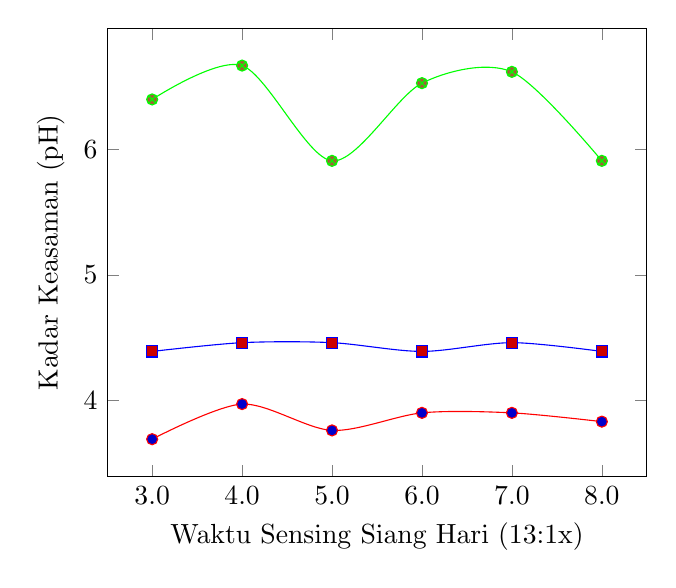
\begin{tikzpicture}[scale=\scl]
		\begin{axis}[\ymin,\ymax,xlabel= Waktu Sensing Siang Hari (13:1x),ylabel=Kadar Keasaman (pH), xticklabel style={/pgf/number format/.cd, fixed,fixed zerofill, precision=1},legend pos = outer north east]
		\addplot+[smooth][color=red] coordinates {(3,3.69) (4,3.97) (5,3.76) (6,3.9) (7,3.9) (8,3.83)};
		\addplot+[smooth][color=blue] coordinates {(3,4.39) (4,4.46) (5,4.46) (6,4.39) (7,4.46) (8,4.39)};
		\addplot+[smooth][color=green] coordinates {(3,6.4) (4,6.67) (5,5.91) (6,6.53) (7,6.62) (8,5.91)};
		\leg
		\end{axis}
		\end{tikzpicture}
		\caption[Kadar Ph Tanah Siang Hari]{Kadar Ph Tanah Siang Hari}
		\label{fig:l1hasil1}
	\end{figure}
    \end{minipage}
    \begin{minipage}[c]{0.49\linewidth}
	\begin{figure}[H]
		\centering
		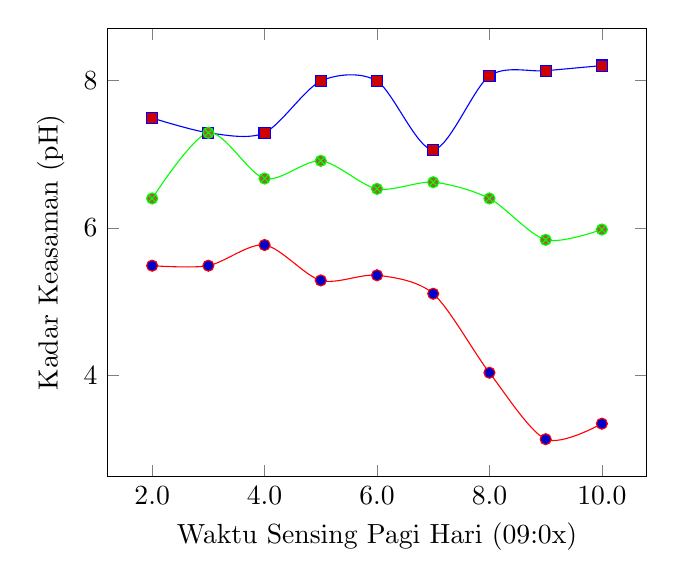
\begin{tikzpicture}[scale=\scl]
		\begin{axis}[\ymin,\ymax,xlabel=Waktu Sensing Pagi Hari (09:0x),ylabel=Kadar Keasaman (pH), xticklabel style={/pgf/number format/.cd, fixed,fixed zerofill, precision=1},legend pos = outer north east]
		\addplot+[smooth][color=red] coordinates {(2,5.49) (3,5.49) (4,5.77) (5,5.29) (6,5.36) (7,5.11) (8,4.04) (9,3.14) (10,3.35)};
		\addplot+[smooth][color=blue] coordinates {(2,7.49) (3,7.29) (4,7.29) (5,7.99) (6,7.99) (7,7.06) (8,8.06) (9,8.13) (10,8.2)};
		\addplot+[smooth][color=green] coordinates {(2,6.4) (3,7.29) (4,6.67) (5,6.91) (6,6.53) (7,6.62) (8,6.40) (9,5.84) (10,5.98)};
		\leg
		\end{axis}
		\end{tikzpicture}
		\caption[Kadar Ph Tanah Pagi Hari]{Kadar Ph Tanah Pagi Hari}
		\label{fig:l1hasil2}
	\end{figure}
\end{minipage}\\

\begin{minipage}[c]{0.49\textwidth}
	\begin{figure}[H]
		\centering
		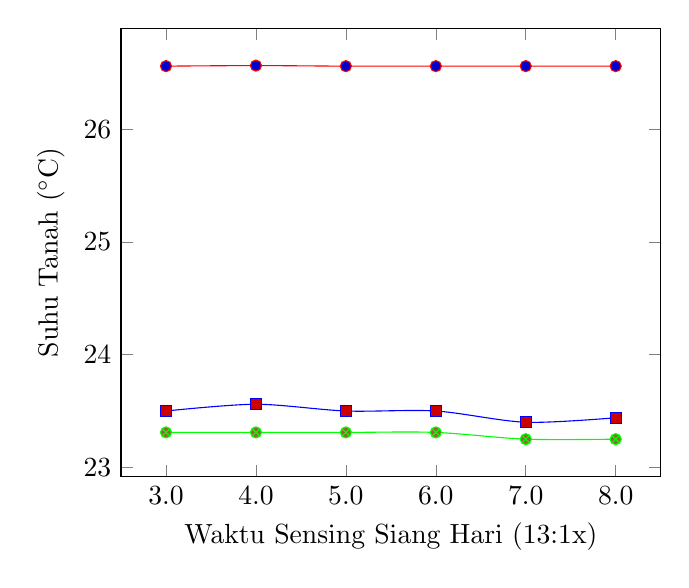
\begin{tikzpicture}[scale=\scl]
		\begin{axis}[\ymin,\ymax,xlabel= Waktu Sensing Siang Hari (13:1x),ylabel=Suhu Tanah ($^{\circ}$C), xticklabel style={/pgf/number format/.cd, fixed,fixed zerofill, precision=1},legend pos = outer north east]
		\addplot+[smooth][color=red] coordinates {(3,26.56) (4,26.565) (5,26.56) (6,26.56) (7,26.56) (8,26.56) };
		\addplot+[smooth][color=blue] coordinates {(3,23.50) (4,23.56) (5,23.50) (6,23.50) (7,23.40) (8,23.44)};
		\addplot+[smooth][color=green] coordinates {(3,23.31) (4,23.31) (5,23.31) (6,23.31) (7,23.25) (8,23.25)};
		\leg
		\end{axis}
		\end{tikzpicture}
		\caption[Suhu Tanah di Siang Hari]{Suhu Tanah di Siang Hari}
		\label{fig:l1hasil1}
	\end{figure}
    \end{minipage}
    \begin{minipage}[c]{0.49\linewidth}
	\begin{figure}[H]
		\centering
		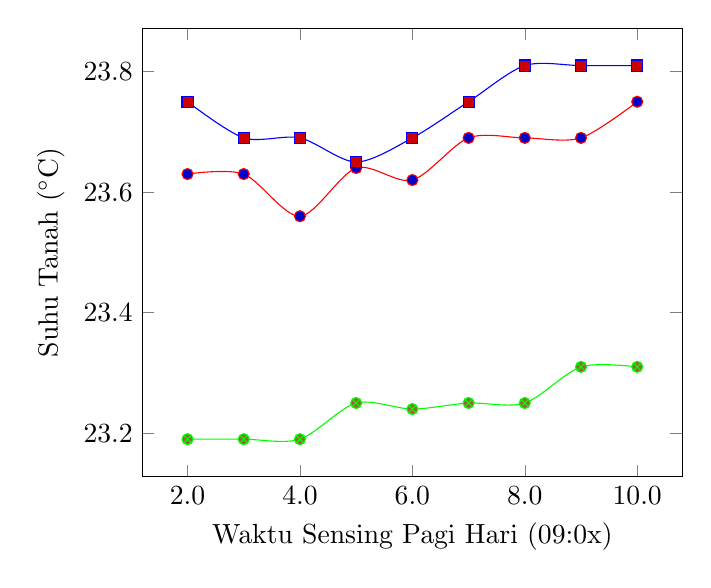
\begin{tikzpicture}[scale=\scl]
		\begin{axis}[\ymin,\ymax,xlabel=Waktu Sensing Pagi Hari (09:0x),ylabel=Suhu Tanah ($^{\circ}$C), xticklabel style={/pgf/number format/.cd, fixed,fixed zerofill, precision=1},legend pos = outer north east]
		\addplot+[smooth][color=red] coordinates {(2,23.63) (3,23.63) (4,23.56) (5,23.64) (6,23.62) (7,23.69) (8,23.69) (9,23.69) (10,23.75)};
		\addplot+[smooth][color=blue] coordinates {(2,23.75) (3,23.69) (4,23.69) (5,23.65) (6,23.69) (7,23.75) (8,23.81) (9,23.81) (10,23.81)};
		\addplot+[smooth][color=green] coordinates {(2,23.19) (3,23.19) (4,23.19) (5,23.25) (6,23.24) (7,23.25) (8,23.25) (9,23.31) (10,23.31)};
		
		\leg
		\end{axis}
		\end{tikzpicture}
		\caption[Suhu Tanah di Pagi Hari]{Suhu Tanah di Pagi Hari}
		\label{fig:l1hasil2}
	\end{figure}
\end{minipage}\\

\begin{minipage}[c]{0.49\textwidth}
	\begin{figure}[H]
		\centering
		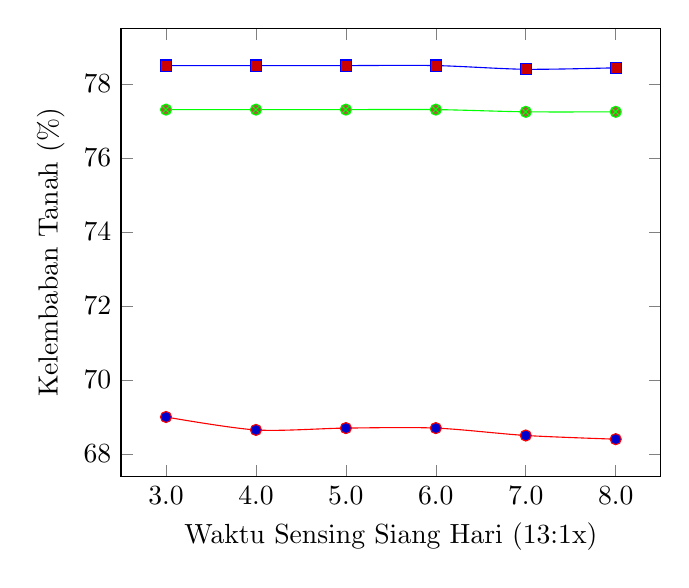
\begin{tikzpicture}[scale=\scl]
		\begin{axis}[\ymin,\ymax,xlabel= Waktu Sensing Siang Hari (13:1x),ylabel=Kelembaban Tanah (\%), xticklabel style={/pgf/number format/.cd, fixed,fixed zerofill, precision=1},legend pos = outer north east]
		\addplot+[smooth][color=red] coordinates {(3,69.00) (4,68.65) (5,68.7) (6,68.7) (7,68.5) (8,68.4) };
		\addplot+[smooth][color=blue] coordinates {(3,78.50) (4,78.5) (5,78.50) (6,78.50) (7,78.40) (8,78.44)};
		\addplot+[smooth][color=green] coordinates {(3,77.31) (4,77.31) (5,77.31) (6,77.31) (7,77.25) (8,77.25)};
		\leg
		\end{axis}
		\end{tikzpicture}
		\caption[Kelembaban Tanah di Siang Hari]{Kelembaban Tanah di Siang Hari}
		\label{fig:l1hasil1}
	\end{figure}
    \end{minipage}
    \begin{minipage}[c]{0.49\linewidth}
	\begin{figure}[H]
		\centering
		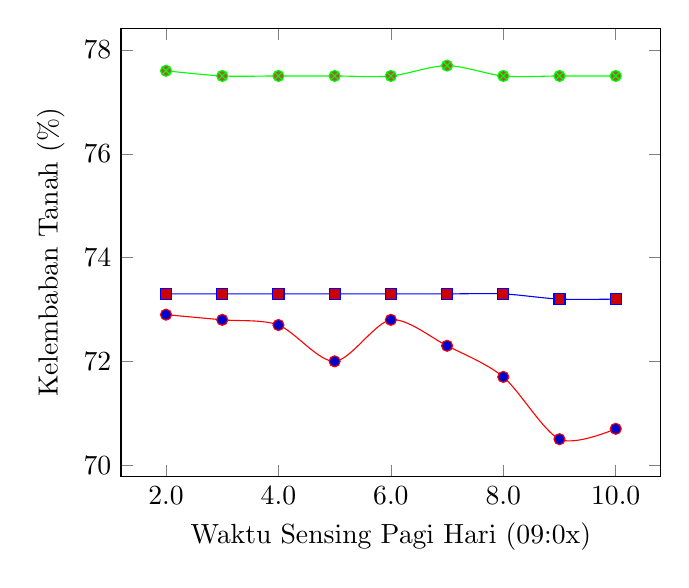
\begin{tikzpicture}[scale=\scl]
		\begin{axis}[\ymin,\ymax,xlabel=Waktu Sensing Pagi Hari (09:0x),ylabel=Kelembaban Tanah (\%), xticklabel style={/pgf/number format/.cd, fixed,fixed zerofill, precision=1},legend pos = outer north east]
		\addplot+[smooth][color=red] coordinates {(2,72.9) (3,72.8) (4,72.7) (5,72.0) (6,72.8) (7,72.3) (8,71.7) (9,70.5) (10,70.7)};
		\addplot+[smooth][color=blue] coordinates {(2,73.3) (3,73.3) (4,73.3) (5,73.3) (6,73.3) (7,73.3) (8,73.3) (9,73.2) (10,73.2)};
		\addplot+[smooth][color=green] coordinates {(2,77.6) (3,77.5) (4,77.5) (5,77.5) (6,77.5) (7,77.7) (8,77.5) (9,77.5) (10,77.5)};
		
		\leg
		\end{axis}
		\end{tikzpicture}
		\caption[Kelembaban Tanah di Pagi Hari]{Kelembaban Tanah di Pagi Hari}
		\label{fig:l1hasil2}
	\end{figure}
\end{minipage}\\

\begin{minipage}[c]{0.49\textwidth}
	\begin{figure}[H]
		\centering
		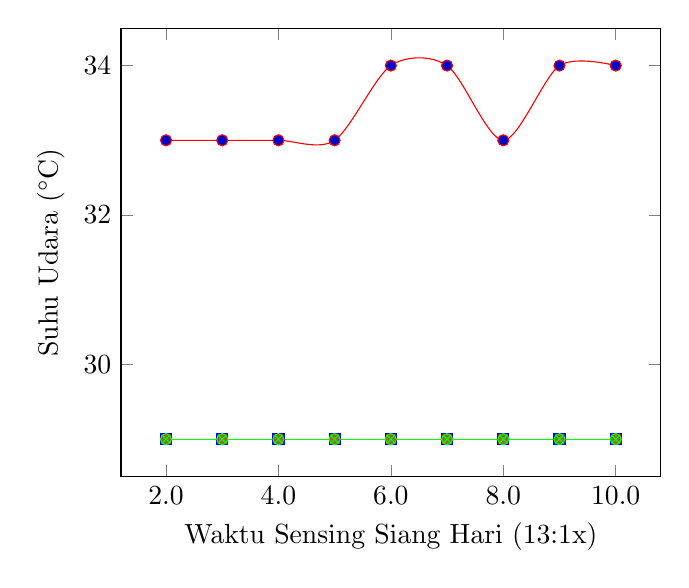
\begin{tikzpicture}[scale=\scl]
		\begin{axis}[\ymin,\ymax,xlabel= Waktu Sensing Siang Hari (13:1x),ylabel=Suhu Udara ($^{\circ}$C), xticklabel style={/pgf/number format/.cd, fixed,fixed zerofill, precision=1},legend pos = outer north east]
        \addplot+[smooth][color=red] coordinates {(2,33) (3,33) (4,33) (5,33) (6,34) (7,34) (8,33) (9,34) (10,34)};
		\addplot+[smooth][color=blue] coordinates {(2,29) (3,29) (4,29) (5,29) (6,29) (7,29) (8,29) (9,29) (10,29)};
		\addplot+[smooth][color=green] coordinates {(2,29) (3,29) (4,29) (5,29) (6,29) (7,29) (8,29) (9,29) (10,29)};
		\leg
		\end{axis}
		\end{tikzpicture}
		\caption[Suhu Udara di Siang Hari]{Suhu Udara di Siang Hari}
		\label{fig:l1hasil1}
	\end{figure}
    \end{minipage}
    \begin{minipage}[c]{0.49\linewidth}
	\begin{figure}[H]
		\centering
		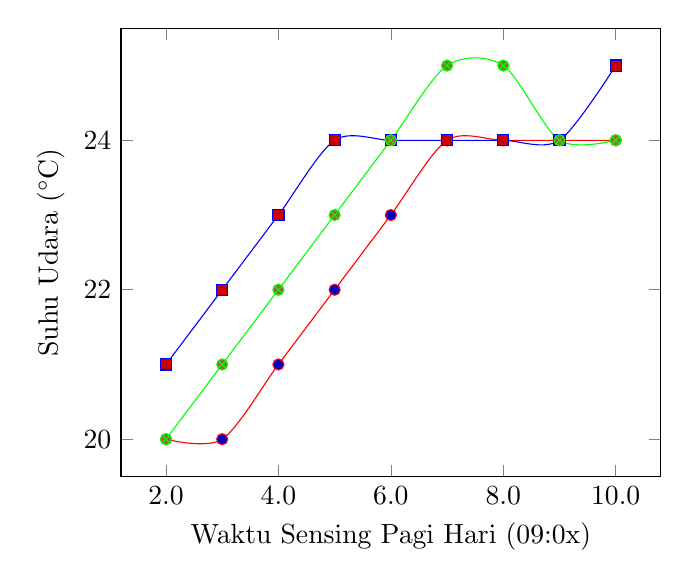
\begin{tikzpicture}[scale=\scl]
		\begin{axis}[\ymin,\ymax,xlabel=Waktu Sensing Pagi Hari (09:0x),ylabel=Suhu Udara ($^{\circ}$C), xticklabel style={/pgf/number format/.cd, fixed,fixed zerofill, precision=1},legend pos = outer north east]
		\addplot+[smooth][color=red] coordinates {(2,20) (3,20) (4,21) (5,22) (6,23) (7,24) (8,24) (9,24) (10,24)};
		\addplot+[smooth][color=blue] coordinates {(2,21) (3,22) (4,23) (5,24) (6,24) (7,24) (8,24) (9,24) (10,25)};
		\addplot+[smooth][color=green] coordinates {(2,20) (3,21) (4,22) (5,23) (6,24) (7,25) (8,25) (9,24) (10,24)};
		\leg
		\end{axis}
		\end{tikzpicture}
		\caption[Suhu Udara di Pagi Hari]{Suhu Udara di Pagi Hari}
		\label{fig:l1hasil2}
	\end{figure}
\end{minipage}\\
    
    Grafik diatas merupakan grafik hasil pemantauan yang memiliki value yang sama dengan tabel \ref{tab:Tabel Pemantauan di Siang Hari} dan tabel \ref{tab:Tabel pemantauan pagi hari}. Grafik berwarna merah merepresentasikan kode node satu, sedangkan grafik berwarna biru dan hijau merepresentasikan kode node dua dan tiga.
    Dari tabel dan grafik diatas, yang merupakan hasil pemantauan yang dilakukan selama dua hari di persawahan milik PT.Pindad persero juga menghasilkan informasi bahwa hujan mempengaruhi kadar keasaaman tanah sawah. Hal ini dapat dibuktikan dengan drastisnya nilai pH tanah yang berada di tabel \ref{tab:Tabel Pemantauan di Siang Hari} yang merupakan data tanah sebelum hujan dengan tabel \ref{tab:Tabel pemantauan pagi hari} yang merupakan data tanah setelah hujan. Selain itu waktu dilakukannya pemantauan juga mempengaruhi nilai suhu ideal dari tanah yang dilakukan pemantauan. 
   
\section{Kendala}
\label{sec:latex}

    Pada pembangunan suatu aplikasi, umumnya akan ditemukan beberapa kendala, baik dari segi pemrograman maupun dari segi perangkat keras yang digunakan. Begitupula pada pembangunan aplikasi pemantauan kualitas tanah sawah yang dibangun.
    
    \subsection{Kendala Pemrograman}
    Berikut adalah kendala atau masalah yang dihadapi selama perancangan dan pembangunan aplikasi dari segi pemrograman.
    
    \begin{itemize}
        \item Pemrograman Node Sensor
        
         Kendala yang dihadapi pada tahap pemrograman adalah bug yang menyebabkan sensor hanya dapat melakukan \textit{sensing} dalam jangka waktu tertentu lalu terhenti. Namun kendala ini telah dituntaskan dengan cara memastikan hasil \textit{sensing} telah dikirim sebelum melakukan \textit{sensing} kembali. Selain itu juga library yang dimiliki oleh Arduino bersifat \textit{fixed} sehingga sulit mengetahui apakah error terjadi di perangkat keras atau kode program.
        
        \item Pemrograman \textit{Base station}
        
        Kendala lain yang dihadapi pada pemrograman pada \textit{base station} adalah banyak mendapatkan kendala untuk interfacing perangkat keras, yang akan dibahas di subbab \ref{kendala perangkat keras}.
        
        
    \end{itemize}
   
   
   \subsection{Kendala Perangkat Keras}
   \label{kendala perangkat keras}
   Berikut adalah kendala atau masalah yang dihadapi selama perancangan dan pembangunan aplikasi dari segi perangkat keras.
   
   \begin{itemize}
       \item Laptop
       
       Ada beberapa kendala yang dihadapi pada perangkat keras laptop, diantaranya adalah kendala dalam melakukan instalasi aplikasi putty dan VCN untuk melakukan \textit{interfacing} dengan perangkat Raspberry Pi berdasarkan jaringan yang terhubung. Selain itu, kendala juga terjadi dalam mencari ip Raspberry Pi yang terhubung dalam jaringan.
       
       \item Raspberry Pi 3 B+
       
       Kendala yang dihadapi pada perangkat Raspberry Pi 3 B+ adalah komunikasi antara Raspberry Pi dengan laptop yang akan menjadi monitor menggunakan perangkat lunak VNC (untuk GUI) atau putty (untuk CLI). Selain itu juga mengakses izin port-port agar perangkat xbee dapat berkomunikasi, serta mengupdate versi php dan menginstall laravel pada perangkat Raspberry Pi yang lebih rumit dibandingkan perangkat laptop. 
       
       
       \item Node Sensor
       
       Hampir tidak ada kendala yang didapat dari node sensor, namun perbedaan kecepatan pengiriman paket hasil \textit{sensing} terjadi antara Arduino \textit{original} dengan yang \textit{non-original}.
       
       \item Sensor \textit{Sensing}
       
       Kendala pada sensor \textit{sensing} adalah adanya beberapa sensor yang memerlukan kegiatan khusus seperti merakit atau menggunakan las untuk menghubungkan kabel.
   \end{itemize}